\documentclass{article}
\usepackage[utf8]{inputenc}
\usepackage{graphicx}
\usepackage{hyperref}

\title{Requirements and Design Document}
\author{TeamTuring:\\\\Darius Scheepers, Kyle Pretorius, Richard Dixie, Sewis van Wyk,\\\\ Tristan Rothman \& Ulrik De Muelenaere\\\\ ERP-Coin}
\date{}

\begin{document}

\maketitle
\begin{center}

\includegraphics[scale=0.1]{erp-logo.png}
\end{center}

\begin{center}

\includegraphics[scale=0.15]{epi-use.png}
\end{center}

\section{System Overview}

\subsection{Purpose}
Non-profit conservation areas rely on volunteers to patrol the area to report suspicious behaviour, injured animals or any violations of the conservation area rules. To encourage more volunteers to patrol these areas in their free time some system needs to be put in place, the ERP-Coin system will not only augment the patrolling experience volunteers but will also reward for their time with ERP-Coins.
 
\subsection{Project Scope}
The ERP Coin system will allow volunteers to view a map of the conservation area they are currently patrolling, this map will show volunteers where other volunteers have recently been allowing them to patrol new routes within the conservation area. The system will also put volunteers in connection with the conservation area managers and other volunteer by allowing them to send alerts, these alerts may be used to report any suspicious behaviour or injured animal. When a volunteer sends an alert the conservation admin will immediately be notified and will be able to broadcast alerts to all volunteers in the area, these alerts will now also appear on their maps. As a reward volunteers always have a random chance of earning an ERP-Coin (see section 1.3) while patrolling, volunteers will have a higher probability of earning coins in areas that have not recently been patrolled.\\\\The system will also provide an interface to conservation area managers to view and broadcast alerts as well as propose new rewards that their conservation area will have available. Lastly ERP (see section 1.3) will have access to an interface allowing them to add new conservation areas and managers to the system as well as verifying rewards proposed by the area managers.
\vspace{2em}
\subsection{Definitions, acronyms and abbreviations}
In this documents the following abbreviations and acronyms will be used:
\begin{itemize}
\item ERP: A bold, non-profit organization called Elephants, Rhinos \& People (ERP) is helping solve one of the world’s tragic problems, with support from SAP.
\item ERC-20: ERC-20 is a technical standard used for smart contracts on the Ethereum blockchain for implementing tokens. ERC stands for Ethereum Request for Comment, and 20 is the number that was assigned to this request.
\item ERP-Coin: The ERC-20 token that will be awarded to users when patrolling conservation areas.
\end{itemize}


\subsection{UML Domain model}
\begin{figure}[!h]
\centering
\makebox[\textwidth]{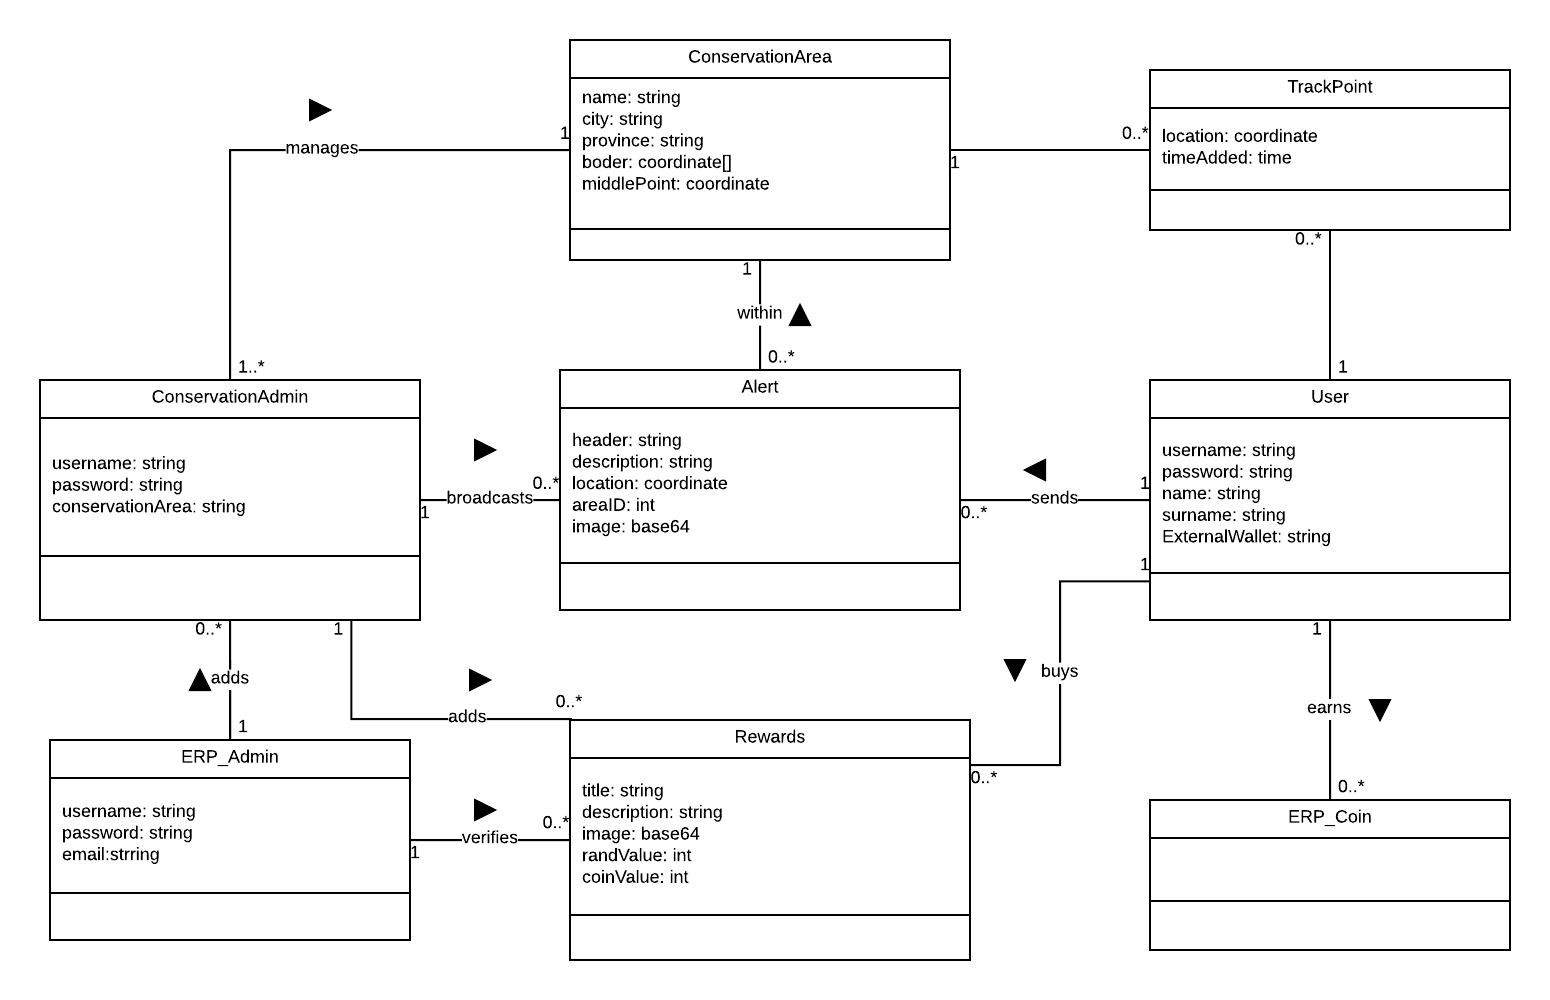
\includegraphics[scale=0.7]{DomainModel.png}}
\caption{Domain model for the system}
\end{figure}

\section{Functional Requirements}

\subsection{Users}
\subsubsection*{Public}
The majority of our users will be anyone who would like to patrol a conservation area to prevent poaching or harm to any of the animals in the area. These users will use our application to select a conservation area they would like to patrol, they will then be able to view alerts that have been sent by other users and conservation admins. The users will also be able to see areas where other users have been which will help them patrol areas that have not been patrolled recently, as a reward for patrolling users always have a chance of finding an ERP-Coin during their patrol with a higher probability for finding a coin in areas that have not been patrolled recently. If a users wishes to alert other users of anything they have seen they will be able to send an alert to an conservation admin with a short description and an image.\\\\These users will also be able to buy rewards from our store with the ERP-Coins that they have earned, these rewards are added by the conservation areas and can include merchandise, food and weekends away at selected areas. Additionally our applications allow users to link an external Ethereum wallet which they can use to keep their ERP-Coins secure or send them to other users.\\\\The application will be easy to use and will not require any technical skills from these users, if users decide to load their ERP-Coins to an external wallet they will have to have knowledge about using Ethereum wallets but this is only an additional feature for advanced users and they application will be fully functional without linking an external wallet.

\subsubsection*{Conservation Area Admins}
Each registered conservation area will have one or more admins associated with it, these admins are usually on site and their main use of our application will be to respond to alerts that have been sent by the public who patrol their area. These users will be able to view a map with all new alerts sent by users, they will then be able to select alerts and either delete them or edit them and broadcast them to the public, making the alert visible to all users patrolling that conservation area.\\\\The conservation admins will also use our application to add rewards available from their area, they will be responsible for giving a brief description of the rewards, an image and a value in rand for the reward(this rand value is only used a guide by the super admin to determine the ERP-Coin value of the reward). Before these rewards become visible to the public they will first have to be verified by the EPI-USE super admin.\\\\The application only assumes that these users are on site and will be able to respond to alerts within a reasonable time, no specific technical skills will be required to use our application to manage the conservation areas.\\

\subsubsection*{ERP super admin}

To allow EPI-USE to manage the use of the application, our application requires that one or more super admins are registered by EPI-USE. These admins are mainly responsible for adding or removing conservation areas from the system as well as assigning conservation area admins to each of the areas. They will also be required to verify new rewards proposed by conservation area admins before they will be visible to the public, this is to ensure that all rewards visible to the public are approved by EPI-USE. Additionally they will assign an ERP-Coin value to each reward, the public will only be able to see the value of rewards in ERP-Coin and not in as a Rand value.\\\\These users must be highly trusted by EPI-USE since they have control over most of the system. They will also be responsible of keeping track of the conversion rate from Rand to ERP-Coin, this rate my change as the number of users that use the application increases and maintaining a good conversation rate is critical to making patrolling from the general public beneficial to the general public while making it affordable to conservation areas. 

\subsection{Subsystems}
The system will consist of three user interfaces which are discussed in section 4.1.1, each of these interfaces can be seen as a logical unit. \\\\Furthermore the system will consist of three logical subsystem that are each responsible for providing different functionality, these subsystems are as follows:
\begin{itemize}
\item Conservation area management:
This system provides the functionality for adding new conservation areas to the database and removing conservation areas.
\item User Patrol tracking:
This system used to keep track of where users have recently been inside conservation areas, this is achieved by storing locations received from the user front end every minute. These locations are store in the database as units referred to as points, the system will provide other system with information about points close to a specific users or the total points in a specific conservation area. Additionally the system will remove points that are older than a day or when the total number of points for an area have exceeded the maximum limit.
\item ERP Token management:
This system is used to award ERP-Coins to users that will be stored in the database as well as send coins to external wallets if the user has decided to link one. Any communication with the block chain contracts will be done by this subsystem.
\item Alert management:
This system is responsible for providing any functionality related to alerts that have been sent by user and conservation area admins, this includes interacting with the database server to store and retrieve alerts from certain conservation areas as well as setting alerts to be broadcasted when requested by conservation admins.
\item Reward management:
This system is responsible for providing any functionality related to rewards available from conservation areas, this includes interacting with database servers to store and retrieve rewards from certain conservation areas as well as setting rewards to be verified when requested by super admins.
\end{itemize} 
Any persistent storage will be handled by the following two subsystems:
\begin{itemize}
\item Database server:
This system is responsible for storing any information relating to conservation areas, alerts sent by users, rewards added by conservation area managers and locations of where users have recently been.
\item Ethereumm blockchain:
The blockchain can be seen as an independent system that provides functionality for storing the coins balances of users who have chosen to link an external ethereum wallet.  
\end{itemize}

\vspace{1em}
\begin{figure}[h]
\centering

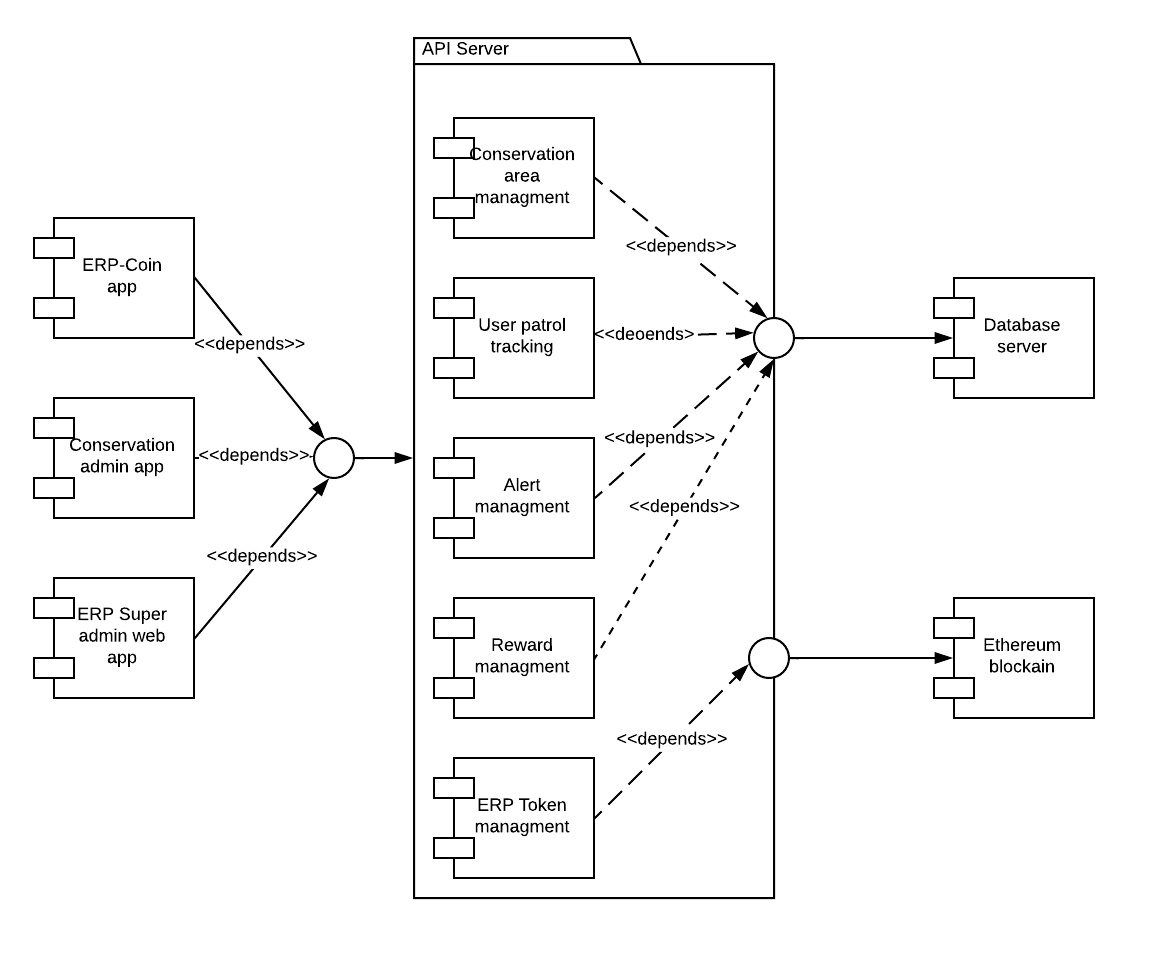
\includegraphics[scale=0.7]{ComponentDiagram.png}
\caption{Component diagram of subsystems}
\end{figure}
\vspace{1em}


\subsection{Specific requirements}
General public users:
\begin{enumerate}
    \item As a user I can create a new account on the mobile application.
    \item As a user I can log in to my account on the mobile application.
    \item As a user I can view a list of available reserves to visit, and select the one I would like to patrol.
    \item As a user I can start patrolling an area using the map on the app.
    \item As a user I can find ERP coins while patrolling.
    \item As a user I can issue an alert when I see something that needs to be reported.
    \item As a user I can view a list of available rewards offered by the nature reserve.
    \item As a user I can use my ERP coins to buy a reward from the nature reserve.
\end{enumerate}
\vspace{3em}
ERP admin:
\begin{enumerate}
    \item As an ERP admin I can log in as a ERP admin on the Web Portal.
    \item As an ERP admin I can add and remove new reserve admins.
    \item As an ERP admin I can add and remove new nature reserves.
    \item As an ERP admin I can approve new rewards that have been proposed by reserve admins.
    \item As an ERP admin I can set ERP-Coin values to rewards visible to the public.
\end{enumerate}
\vspace{2em}
Reserve admin:
\begin{enumerate}
    \item As a reserve admin I can log in as a reserve admin on the app.
    \item As a reserve admin I can view and broadcast alerts issued by users patrolling the reserve I manage.
    \item As a reserve admin I can add new alerts that will be visible to the public.
    \item As a reserve admin I can propose new rewards that will be offered by the reserve.
\end{enumerate}
\begin{figure}[h]
\centering
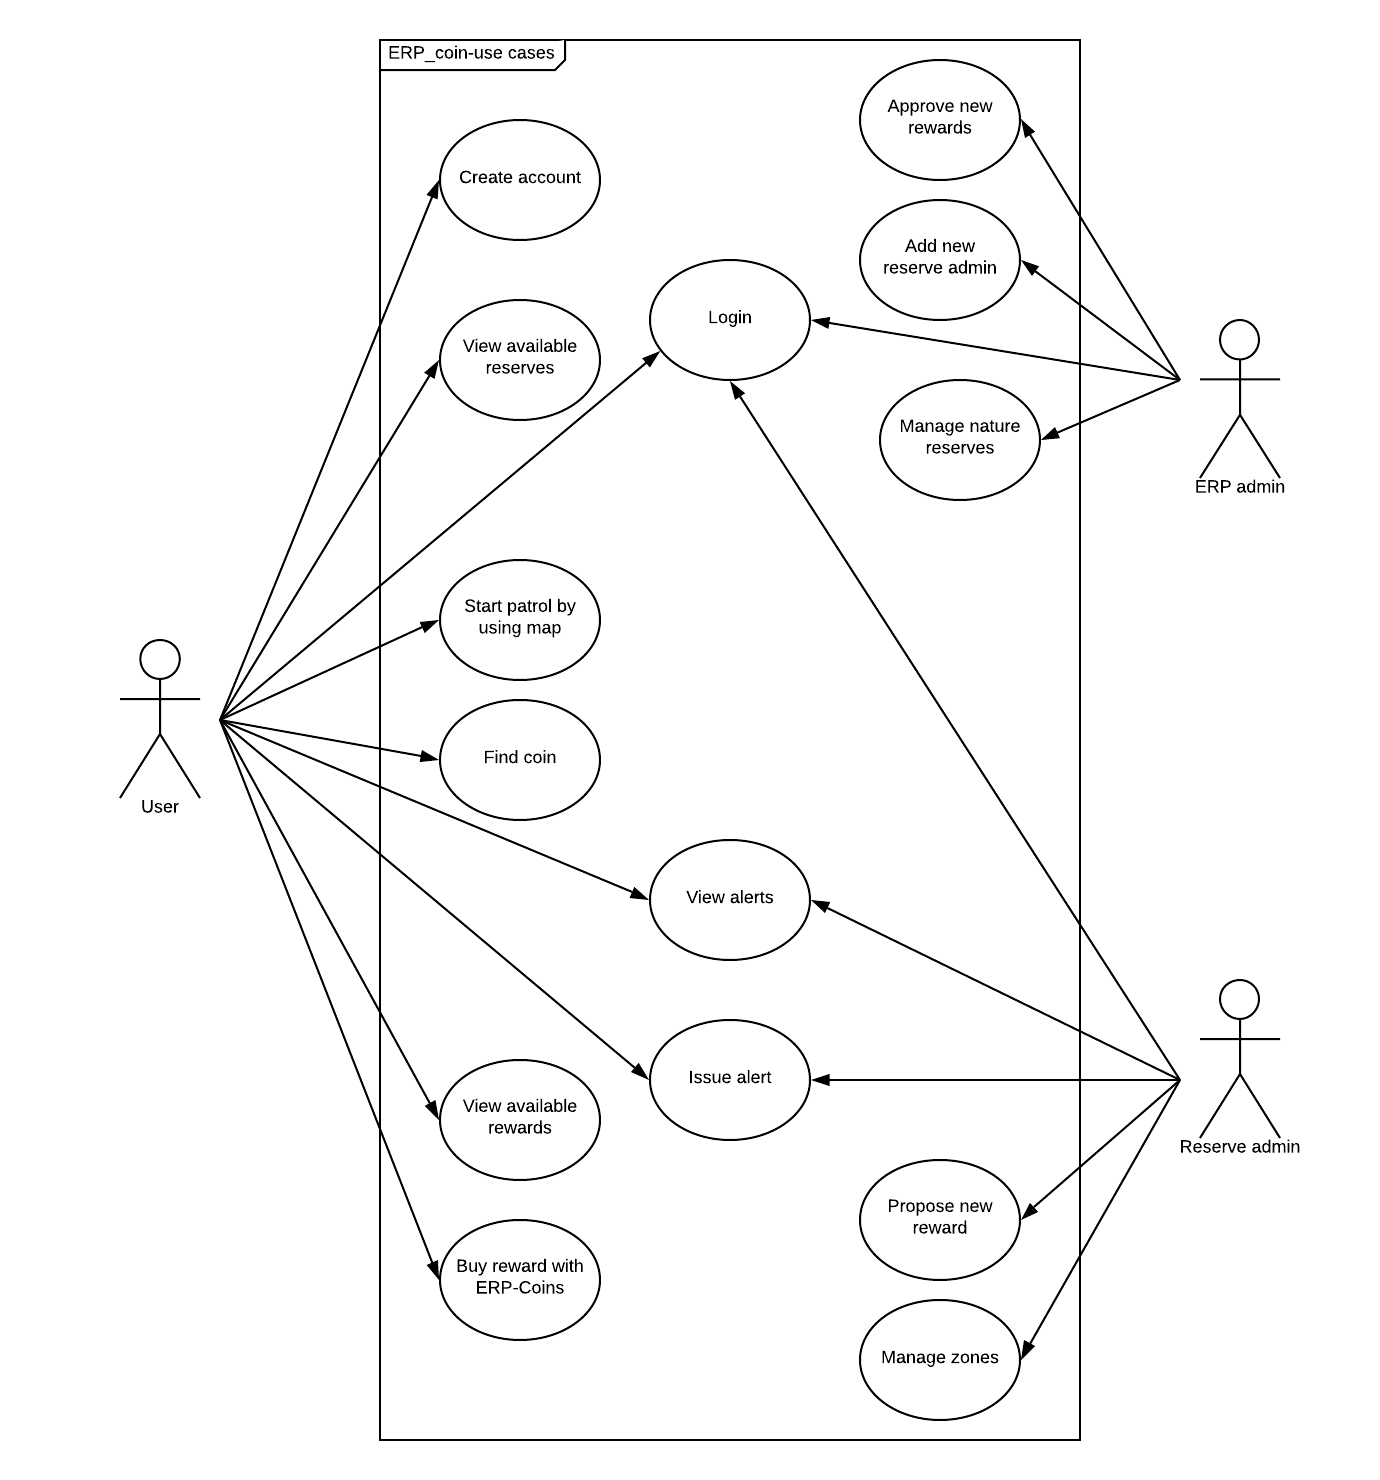
\includegraphics[scale=0.5]{UseCase.png}
\caption{Use case diagram for functional requirements}
\end{figure}

\section{Non-functional requirements}
\subsection{Usability}
\begin{itemize}
\item Importance: The success of the application depends on the general public patrolling conservation areas in their free time. This means that it is important for the user to have a pleasant experience when using the application, our application must be simple to use since users will be using it on the move. 
\item How it is achieved: The application will have very simple and intuitive user interfaces. The user interfaces must clearly show the main functionality presented by that interface without being too cluttered since users will have to use the application while walking and will not want to spend too much time looking down on their screen. The user interface used by the public will have a large map on the interface used for patrolling with colour coded alerts indicating the severity of the alert, as the user moves blue dots will be plotted showing were other users have recently been.
\end{itemize}

\subsection{Security}
\begin{itemize}
\item Importance: The application will contain a rewards system rewarding ERP-Coin to users, since these coins will have a monetary value its is important to ensure that all transactions relating to these coins are very secure. The application should prevent any user from exploiting any interface or request to the server to receive or intercept coins being transacted.
\item How it is achieved: Security is achieved by encapsulating any subsystems that are responsible for allocating or sending coins in a separate layer, additionally any communication with this layer is controlled by a separate layer called the application layer. Since users will only have access to the interfaces part of the presentation layer, any request they sent will be handled and validated by the application layer and the application layer will communicate with the database layer, 
\end{itemize}

\subsection{Portability}
\begin{itemize}
\item Importance: Users will be free to use the application on any web browser of their choice, this is important because the success of the application depends on the number of users that use it. Restricting users to use certain web browsers will result in less users using the application since they will be required to install the required web browser. 
\item How it is achieved: The first factor that greatly contributes to portability is the use of a web application instead of a native application, web applications do not require users to use an app store to be installed, users can simply visit the website and use the add to home screen functionality to easily access the application from their home screen. The second that contributes to portability is the use of framework such as ionic that builds web applications that can be used on many different web browsers, allowing users to use the web browser of their choice.
\end{itemize}
\vspace{4em}
\section{System architecture}

\subsection{Interfaces}
 
\def\sectionautorefname{UI}
The system will provide three User Interfaces, one for each of the three categories of users listed in section 2.1. The purpose of each user interface directly corresponds to the requirements listed in section 2.3.

\begin{itemize}
\item ERP-Coin app:\\
This user interface will be used by the general public to patrol a conservation area, the interface will provide a screen with a large map showing the border of the conservation area they are currently patrolling. Alerts sent be other users and admins will also be visible on the map and if clicked on will display a short description as well as an image relating to the alert if provided. Users will also be able to send alerts for which they will add a short description and attach a photo. Users will be notified every time they have earned a coin during the patrol. The interface will also contain a store that users can use to view available rewards on conservation areas and purchase rewards with ERP-Coins they have earned. An option to link an external wallet to which they wish to transfer their ERP-Coins to will also be provided.\\

\item Conservation area admin app:\\
This interface will be used by Conservation area admins, the interface allows admins to view all alerts that have been broadcasted as well as new alerts recently sent my users. The admins will be able to verify these alerts, edit them and choose to broadcast them to all the users. Lastly the interface will allow admins to suggest new rewards for the conservation area they are assigned to, they will be able to set a description, image and rand value for each reward they list.

\item ERP Super admin web interface:\\
This interface will be used by ERP admins assigned by EPI-USE, the interface will allow admins to add new conservation areas and register new conservation area admins for each area. They will also be able to view and modify rewards that are visible to the public and verify new rewards proposed by conservation area admins before they are visible to the public.
\end{itemize}

\subsubsection{Hardware interfaces}
The following ports will be used by the system:
\begin{itemize}
\item 443: Web server for hosting the user interfaces.
\item 8080: Requests from front-end user interfaces to back-end server via HTTPS.
\item 3306: SQL server for storing and manipulating data as requested by back-end server.
\item 8545: JSON-RPC for requests between from the front-end and back-end server to the Ethereum blockchain.
\end{itemize}

The following hardware will be used on mobile devices:
\begin{itemize}
\item Mobile application requires access to file system and/or camera for uploading images to the system.
\item Mobile application requires access to GPS for live location tracking.
\end{itemize}

\subsubsection{Software interfaces}
The following two external API's are used by the system:
\begin{itemize}
\item Google Maps: Used by user interfaces require this API to display maps of conservation areas as well as the live location of users currently patrolling.
\item Open Street Map: Used by the ERP-Admin user interface when adding new conservation areas, this API is used to automatically retrieve border points of conservation areas to reduce the burden on admins.
\end{itemize}
\subsection{Architectural styles}
The system has been designed as a three tier architecture. The system will need to be highly interactive and constantly respond to user request while also tracking them during this patrol. This architecture allows for the user system to consist of three sub components the Presentation layer, the Application layer and the Data layer. This creates low coupling between these subsystems allowing each one to function on a different device. The Presentation layer will run on the user device while the Application layer will run om a central node while the Data layer will run on a secure remote site.\\\\The Presentation layer will consist of three interfaces each used by different actors. The first is the User mobile interface called ERP coin that will be used by users to patrol the reserve and earn coins. The second interface will be used by ERP administrators to manage reserves and approve new rewards. The third interface will be used by Reserve admins to view alerts issued and propose new rewards to ERP admins. All three of these user interfaces will only communicate with the application layer and never directly with the database layer for security reasons.\\\\The Application layer will consist of three components, the first of which is the Area management, this component will be responsible for rendering area borders and keeping track of how often areas within the reserve have been patrolled. The second component is the Patrol tracking, which is responsible for tracking the current locations of active users and notifying the area management as well as adding new conservation areas by admins. The last component is the token management that will be responsible for issuing new tokens to users as they patrol and allowing users to buy rewards using their tokens. Both the Area management and Token management will be rely on constant feedback from the Patrol tracking, for this reason it is important that all three these components run on the same machine. The area management and token management will access the Database layers interface when needed.\\\\The Database layer will consist of a server on which the database is run which is used to store information about users, rewards and areas. It will also be used as a wrapper for the Ethereum blockchain, on which the token will be stored. This layer will only be accessed by the application layer to ensure that the data stored on this server is secure.\\\\See figure 4 for a package diagram of the system architecture.

\vspace{2em}
\begin{figure}[h]
\centering
\makebox[\textwidth]{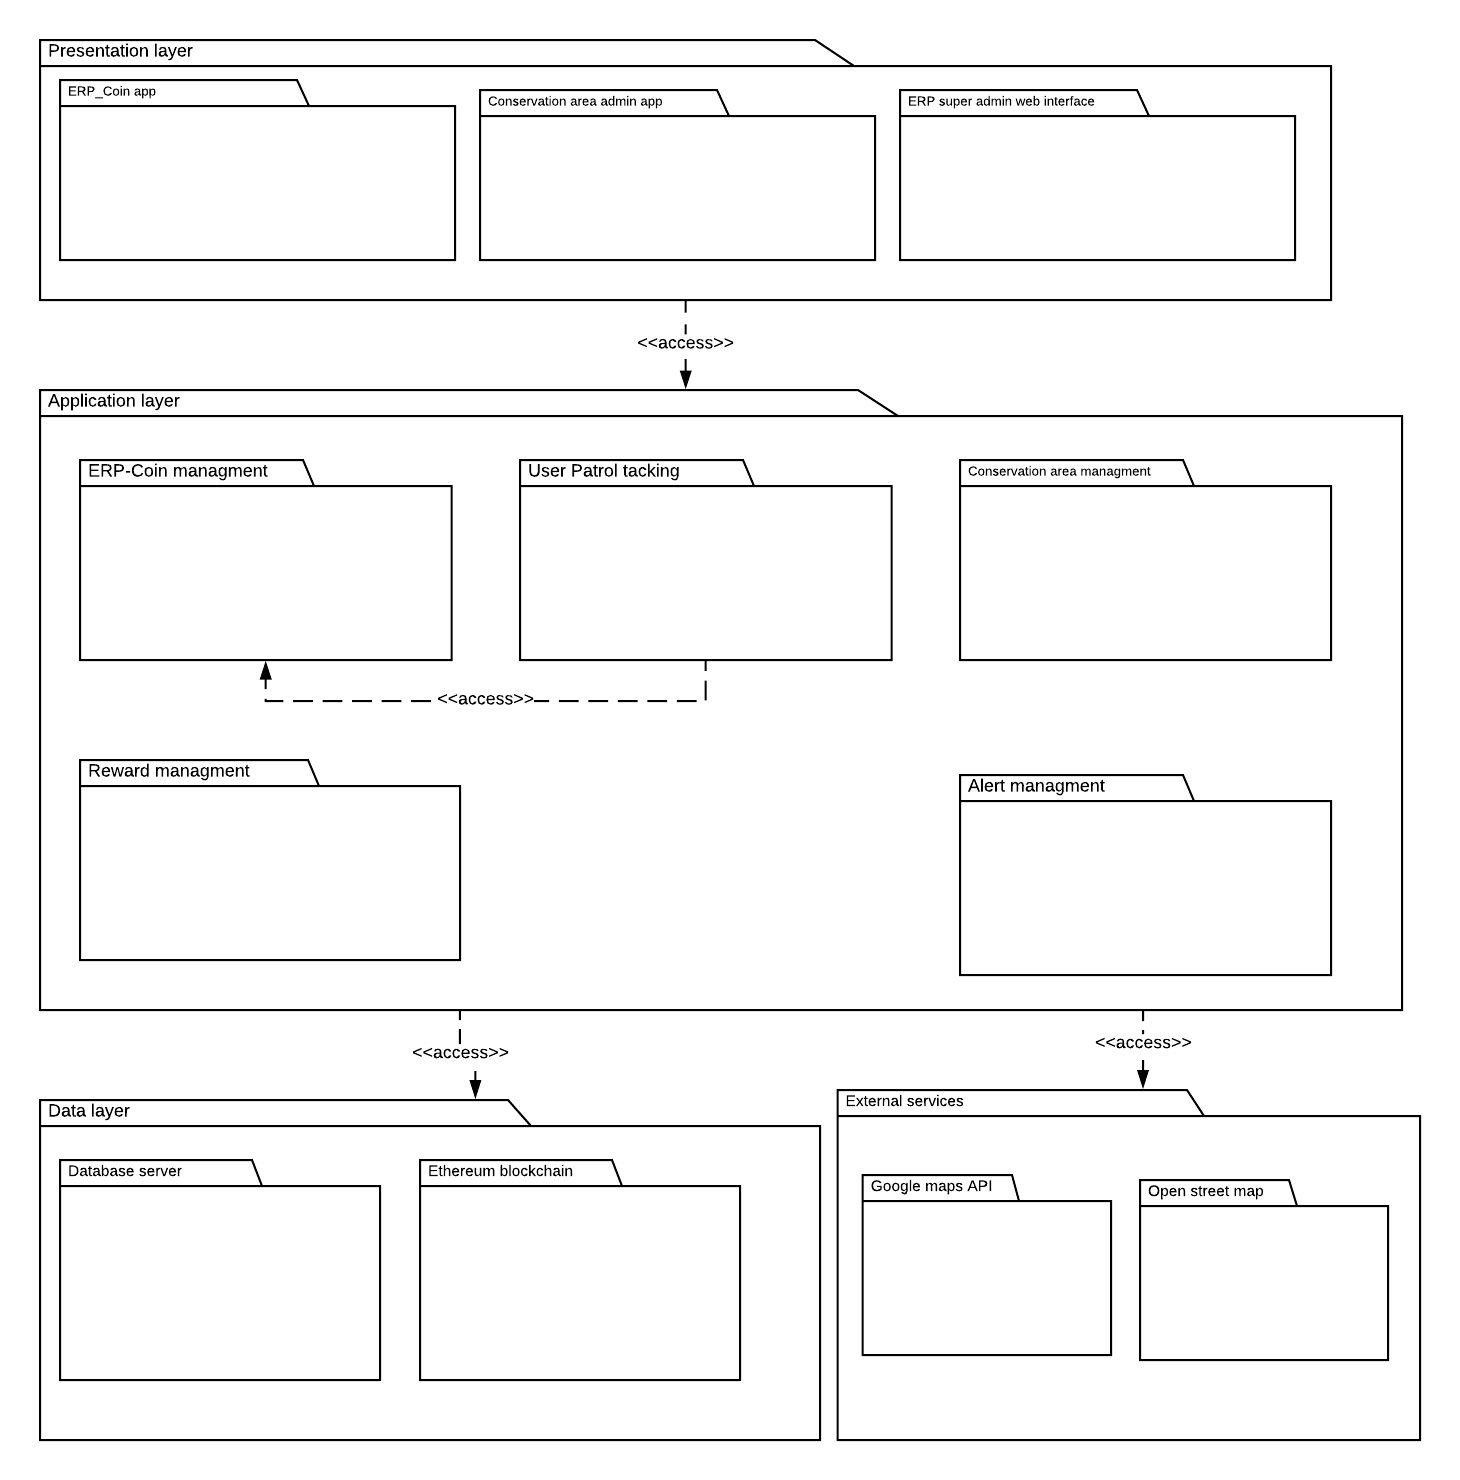
\includegraphics[scale=0.7]{PackageDiagram.png}}
\caption{Package diagram for system architecture}
\end{figure}

\subsection{System configuration}

\subsubsection*{Equipment}
\begin{itemize}
\item The system requires a server computer, to run the Application Layer server
\begin{itemize}
\item Minimum Hardware requirements
\begin{itemize}
\item Memory: Minimum 2GB RAM DDR3/DDR4
\item Processor: 4-Thread CPU
\item Storage: 500GB Hard Drive 
\end{itemize}
\item Software requirements
\begin{itemize}
\item Any operating system that can run a Node.js server, a MySQL server and a Geth Node
\item Node.js Server, version 10.10.0
\item MySQL Server, version 8.0
\item Geth, version 1.8.15 (To run the Ethereum Node)
\end{itemize}
\item Configuration
\begin{itemize}
\item Node.js dependencies need to be installed via npm
\item The Node.js server needs to be configured to connect to the MySQL Database
\item The Node.js server needs to be configured to connect to the Geth Node
\item Geth needs to be run to gain access to the Ethereum Blockchain
\item Contracts need to be deployed via Truffle (one of the npm dependencies)
\item Certificates need to be configured to serve over HTTPS
\end{itemize}
\end{itemize}
\item The system requires a computer to run all of the user interfaces. These interfaces can also run on the Application Layer server mentioned above
\begin{itemize}
\item Minimum Hardware requirements
\begin{itemize}
\item Memory: Minimum 2GB RAM DDR3/DDR4
\item Processor: 2-Thread CPU
\item Storage: 125GB Hard Drive
\end{itemize} 
\item Software requirements
\begin{itemize}
\item Any operating system that can run a HTTP server
\end{itemize}
\item Configuration
\begin{itemize}
\item Certificates need to be configured to serve over HTTPS
\end{itemize}
\end{itemize}
\item The clients require a mobile device, or a computer, to access the interfaces. The only requirement for these devices, is that the device must be capable of web browsing
\end{itemize}

\subsubsection*{Communications}
\begin{itemize}
\item JSON-RPC
\begin{itemize}
\item JavaScript Object Notation Remote Procedure Calls are used for communication between the API (The Application Layer server) and Geth (The Ethereum Node)
\end{itemize}

\item HTTPS for client-API
\begin{itemize}
\item Hyper Text Transfer Protocol Secure requests are used for communication between the user web interfaces (The Presentation Layer) and the API (The Application Layer)
\item This is also used to serve the user interfaces (via HTTPS)
\end{itemize}

\item SQL
\begin{itemize}
\item Structured Query Language queries are used to communicate between the API (The Application Layer) and the MySQL Database (The Database Layer)
\end{itemize}

\end{itemize}

\subsubsection*{Networks}
\begin{itemize}
\item The aforementioned communication methods (JSON-RPC, HTTPS and SQL) are all run over the Transmission Control Protocol over Internet Protocol (TCP/IP) 
\end{itemize}


\begin{figure}[h]
\centering
\makebox[\textwidth]{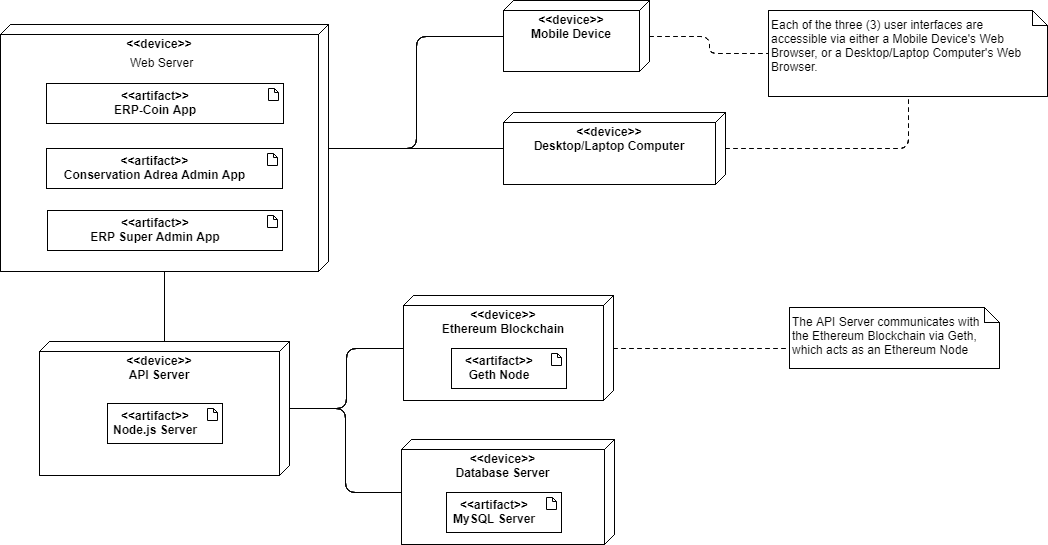
\includegraphics[scale=0.55]{DeploymentDiagram.png}}
\caption{Deployment diagram of system configuration}
\end{figure}

\end{document}